%<dscrpt>Fichier de déclarations Latex à inclure au début d'un élément de cours.</dscrpt>

\documentclass[a4paper]{article}
\usepackage[hmargin={1.8cm,1.8cm},vmargin={2.4cm,2.4cm},headheight=13.1pt]{geometry}

%includeheadfoot,scale=1.1,centering,hoffset=-0.5cm,
\usepackage[pdftex]{graphicx,color}
\usepackage[french]{babel}
%\selectlanguage{french}
\addto\captionsfrench{
  \def\contentsname{Plan}
}
\usepackage{fancyhdr}
\usepackage{floatflt}
\usepackage{amsmath}
\usepackage{amssymb}
\usepackage{amsthm}
\usepackage{stmaryrd}
%\usepackage{ucs}
\usepackage[utf8]{inputenc}
%\usepackage[latin1]{inputenc}
\usepackage[T1]{fontenc}


\usepackage{titletoc}
%\contentsmargin{2.55em}
\dottedcontents{section}[2.5em]{}{1.8em}{1pc}
\dottedcontents{subsection}[3.5em]{}{1.2em}{1pc}
\dottedcontents{subsubsection}[5em]{}{1em}{1pc}

\usepackage[pdftex,colorlinks={true},urlcolor={blue},pdfauthor={remy Nicolai},bookmarks={true}]{hyperref}
\usepackage{makeidx}

\usepackage{multicol}
\usepackage{multirow}
\usepackage{wrapfig}
\usepackage{array}
\usepackage{subfig}


%\usepackage{tikz}
%\usetikzlibrary{calc, shapes, backgrounds}
%pour la présentation du pseudo-code
% !!!!!!!!!!!!!!      le package n'est pas présent sur le serveur sous fedora 16 !!!!!!!!!!!!!!!!!!!!!!!!
%\usepackage[french,ruled,vlined]{algorithm2e}

%pr{\'e}sentation du compteur de niveau 2 dans les listes
\makeatletter
\renewcommand{\labelenumii}{\theenumii.}
\renewcommand{\thesection}{\Roman{section}.}
\renewcommand{\thesubsection}{\arabic{subsection}.}
\renewcommand{\thesubsubsection}{\arabic{subsubsection}.}
\makeatother


%dimension des pages, en-t{\^e}te et bas de page
%\pdfpagewidth=20cm
%\pdfpageheight=14cm
%   \setlength{\oddsidemargin}{-2cm}
%   \setlength{\voffset}{-1.5cm}
%   \setlength{\textheight}{12cm}
%   \setlength{\textwidth}{25.2cm}
   \columnsep=1cm
   \columnseprule=0.5pt

%En tete et pied de page
\pagestyle{fancy}
\lhead{MPSI-\'Eléments de cours}
\rhead{\today}
%\rhead{25/11/05}
\lfoot{\tiny{Cette création est mise à disposition selon le Contrat\\ Paternité-Pas d'utilisations commerciale-Partage des Conditions Initiales à l'Identique 2.0 France\\ disponible en ligne http://creativecommons.org/licenses/by-nc-sa/2.0/fr/
} }
\rfoot{\tiny{Rémy Nicolai \jobname}}


\newcommand{\baseurl}{http://back.maquisdoc.net/data/cours\_nicolair/}
\newcommand{\urlexo}{http://back.maquisdoc.net/data/exos_nicolair/}
\newcommand{\urlcours}{https://maquisdoc-math.fra1.digitaloceanspaces.com/}

\newcommand{\N}{\mathbb{N}}
\newcommand{\Z}{\mathbb{Z}}
\newcommand{\C}{\mathbb{C}}
\newcommand{\R}{\mathbb{R}}
\newcommand{\D}{\mathbb{D}}
\newcommand{\K}{\mathbf{K}}
\newcommand{\Q}{\mathbb{Q}}
\newcommand{\F}{\mathbf{F}}
\newcommand{\U}{\mathbb{U}}
\newcommand{\p}{\mathbb{P}}


\newcommand{\card}{\mathop{\mathrm{Card}}}
\newcommand{\Id}{\mathop{\mathrm{Id}}}
\newcommand{\Ker}{\mathop{\mathrm{Ker}}}
\newcommand{\Vect}{\mathop{\mathrm{Vect}}}
\newcommand{\cotg}{\mathop{\mathrm{cotan}}}
\newcommand{\sh}{\mathop{\mathrm{sh}}}
\newcommand{\ch}{\mathop{\mathrm{ch}}}
\newcommand{\argsh}{\mathop{\mathrm{argsh}}}
\newcommand{\argch}{\mathop{\mathrm{argch}}}
\newcommand{\tr}{\mathop{\mathrm{tr}}}
\newcommand{\rg}{\mathop{\mathrm{rg}}}
\newcommand{\rang}{\mathop{\mathrm{rg}}}
\newcommand{\Mat}{\mathop{\mathrm{Mat}}}
\newcommand{\MatB}[2]{\mathop{\mathrm{Mat}}_{\mathcal{#1}}\left( #2\right) }
\newcommand{\MatBB}[3]{\mathop{\mathrm{Mat}}_{\mathcal{#1} \mathcal{#2}}\left( #3\right) }
\renewcommand{\Re}{\mathop{\mathrm{Re}}}
\renewcommand{\Im}{\mathop{\mathrm{Im}}}
\renewcommand{\th}{\mathop{\mathrm{th}}}
\newcommand{\repere}{$(O,\overrightarrow{i},\overrightarrow{j},\overrightarrow{k})$}
\newcommand{\cov}{\mathop{\mathrm{Cov}}}

\newcommand{\absolue}[1]{\left| #1 \right|}
\newcommand{\fonc}[5]{#1 : \begin{cases}#2 \rightarrow #3 \\ #4 \mapsto #5 \end{cases}}
\newcommand{\depar}[2]{\dfrac{\partial #1}{\partial #2}}
\newcommand{\norme}[1]{\left\| #1 \right\|}
\newcommand{\se}{\geq}
\newcommand{\ie}{\leq}
\newcommand{\trans}{\mathstrut^t\!}
\newcommand{\val}{\mathop{\mathrm{val}}}
\newcommand{\grad}{\mathop{\overrightarrow{\mathrm{grad}}}}

\newtheorem*{thm}{Théorème}
\newtheorem{thmn}{Théorème}
\newtheorem*{prop}{Proposition}
\newtheorem{propn}{Proposition}
\newtheorem*{pa}{Présentation axiomatique}
\newtheorem*{propdef}{Proposition - Définition}
\newtheorem*{lem}{Lemme}
\newtheorem{lemn}{Lemme}

\theoremstyle{definition}
\newtheorem*{defi}{Définition}
\newtheorem*{nota}{Notation}
\newtheorem*{exple}{Exemple}
\newtheorem*{exples}{Exemples}


\newenvironment{demo}{\renewcommand{\proofname}{Preuve}\begin{proof}}{\end{proof}}
%\renewcommand{\proofname}{Preuve} doit etre après le begin{document} pour fonctionner

\theoremstyle{remark}
\newtheorem*{rem}{Remarque}
\newtheorem*{rems}{Remarques}

\renewcommand{\indexspace}{}
\renewenvironment{theindex}
  {\section*{Index} %\addcontentsline{toc}{section}{\protect\numberline{0.}{Index}}
   \begin{multicols}{2}
    \begin{itemize}}
  {\end{itemize} \end{multicols}}


%pour annuler les commandes beamer
\renewenvironment{frame}{}{}
\newcommand{\frametitle}[1]{}
\newcommand{\framesubtitle}[1]{}

\newcommand{\debutcours}[2]{
  \chead{#1}
  \begin{center}
     \begin{huge}\textbf{#1}\end{huge}
     \begin{Large}\begin{center}Rédaction incomplète. Version #2\end{center}\end{Large}
  \end{center}
  %\section*{Plan et Index}
  %\begin{frame}  commande beamer
  \tableofcontents
  %\end{frame}   commande beamer
  \printindex
}


\makeindex
\begin{document}
\noindent

\debutcours{Nombres complexes et trigonométrie}{1.9. \tiny{\today}}

Ce chapitre fait partie du programme de début d'année. Il contient du vocabulaire qui ne sera introduit que plus tard pour éviter des listes fastidieuses de définition en début d'année. On peut se rapporter au \href{\baseurl C4199.pdf}{glossaire de début d'année} pour obtenir des présentations de ces termes mais ce n'est pas indispensable.

Pour manipuler facilement les nombres complexes, il faut absolument éviter de les considérer comme des couples de nombres réels. Les parties réelles et imaginaires sont des propriétés importantes d'un complexe mais il ne faut pas les considérer systématiquement. Le concept le plus délicat est celui d'argument. Il convient de retenir qu'un nombre complexe non nul admet une infinité d'arguments et ne jamais parler de \emph{l'} argument d'un nombre complexe mais \emph{d'un} argument. 

\section{Présentation axiomatique }
Une présentation axiomatique permet d'introduire un objet mathématique sans le définir mais en présentant les propriétés qui le caractérisent et qui permettent de l'utiliser. Cette méthode sera utilisée plusieurs fois dans ce cours et en organisant les propriétés sous la forme \og C'est bien \fg~, \og C'est plus gros que \fg~, \og C'est pas trop gros\fg~ qui permet d'insérer le nouvel objet parmi ceux déjà connus.  
\begin{pa}
 \item[$\C$ c'est bien] : $\C$ est un anneau\footnote{voir l'entrée anneaux-corps du \href{\baseurl C4199.pdf}{glossaire de début d'année}. Un anneau est un ensemble muni de deux opérations (disons une addition et une multiplication) avec des propriétés raisonnables.} contenant un élément particulier noté $i$ tel que 
\begin{displaymath}
 i^2 = -1
\end{displaymath}
\item[$\C$ c'est plus gros que $\R$] : $\R$ est un sous-anneau de  $\C$  et $i$ n'appartient pas à $\R$.
\item[$\C$ c'est pas trop gros] : pour tout nombre complexe $z$, il existe des nombres réels $a$ et $b$ tels que 
\begin{displaymath}
 z = a + i b
\end{displaymath}
\end{pa}
La question de la construction effective d'un modèle pour l'ensemble $\C$ et ses opérations ne sera pas abordée. Ce qu'\og est\fg~  un nombre complexe n'est pas important. Ce qui compte c'est ce qu'on peut faire avec.
La question de l'\og unicité\fg~  revient en fait à prouver qu'entre deux structures vérifiant les propriétés de la présentation axiomatique, il existe un unique isomorphisme. Elle ne sera pas abordée non plus.\newline
En revanche dans le troisième axiome, le fait que, pour un nombre complexe $z$ donné, il existe un \emph{unique} couple de réels est une propriété fondamentale dans la pratique. Ce cours commence par la démonstration de cette proposition. Elle illustre bien les propriétés de $\R$ intervenant dans la présentation axiomatique de $\C$.\index{question de cours : unicité de la décomposition en parties réelles et imaginaires}
\begin{prop}
 Soient $a$, $b$, $a^\prime$, $b^\prime$ des nombres réels tels que 
\begin{displaymath}
 a + ib = a^\prime + i b^\prime
\end{displaymath}
alors $a=a^\prime$ et $b=b^\prime$
\end{prop}
\begin{demo}
 D'après les règles de calcul usuelles (dans un anneau), l'hypothèse entraine $a-a^\prime = i(b^\prime - b)$.\newline
Si $b^\prime - b \neq 0$ alors (propriétés du corps $\R$) c'est un élément inversible. Il existe donc $c\in \R$ tel que :
\begin{displaymath}
 (a-a^\prime)c=i(b^\prime - b)c=i
\end{displaymath}
 Ceci entraine que $i\in \R$ ce qui est impossible car d'après les propriétés de $\R$, aucun réel n'est de carré strictement négatif. On en déduit que $b^\prime - b = 0$ ce qui entraine $a - a^\prime = 0$ et ce qu'on voulait démontrer.
\end{demo}
\index{partie réelle et imaginaire}
\begin{prop}[Parties réelle et imaginaire]
 Pour tout nombre complexe $z$, il existe un unique couple $(a,b)$ de réels tels que 
\begin{displaymath}
 z = a + i b
\end{displaymath}
\end{prop}
\begin{defi}
Les fonctions partie réelle (notée $\Re$) et partie imaginaire (notée $\Im$) sont définies à l'aide de la proposition précédente par :
\begin{displaymath}
 \forall z \in \C : z =\Re z + i \Im z
\end{displaymath}
\end{defi}
Il est à noter que malgré son nom, la fonction \og partie imaginaire\fg~  est à valeurs réelles.
\begin{prop}[Effet des opérations sur les parties réelles et imaginaires] 
 Pour tous $z$ et  $z^\prime$ dans $\C$, pour tout $\lambda$ réel
\begin{displaymath}
\left\lbrace 
\begin{aligned}
 \Re (z + z^\prime) &= \Re (z) + \Re(z^\prime) \\ \Re(\lambda z) &= \lambda \Re(z)
\end{aligned}
\right. 
\hspace{0.5cm}
\left\lbrace 
\begin{aligned}
 \Im (z + z^\prime) &= \Im (z) + \Im(z^\prime) \\  \Im(\lambda z) &= \lambda \Im(z)
\end{aligned}
\right. 
\hspace{0.5cm}
\left\lbrace 
\begin{aligned}
 \Re (z  z^\prime) &= \Re (z) \Re(z^\prime) - \Im (z) \Im(z^\prime) \\
 \Im(z z') &= \Re(z)\Im(z')+\Im(z)\Re(z')
\end{aligned}
\right. 
\end{displaymath}
\end{prop}
Les deux premières accolades traduisent le fait que les fonction $\Re$ et $\Im$ sont \emph{linéaires}.\newline
\index{conjugué d'un nombre complexe}
Les fonctions partie réelle et partie imaginaire permettent de définir la fonction \emph{conjugaison}.
\begin{defi}
 Le conjugué d'un nombre complexe quelconque $z$ est défini par :
\begin{align*}
 \overline{z} = \Re z - i \Im z
\end{align*}
\end{defi}
\begin{prop}[Compatibilité de la conjugaison avec les opérations]
 Pour tous $z$ et  $z^\prime$ dans $\C$, 
\begin{align*}
 \overline{z+z^\prime} = \overline{z} + \overline{z^\prime} & &
\overline{z z^\prime} = \overline{z}  \overline{z^\prime} & &
 \overline{\overline{z}} = z \\
\Re z = \dfrac{1}{2}(z+\overline{z}) & &
\Im z = \dfrac{1}{2i}(z-\overline{z}) & &
z\overline{z} = \Re(z)^2+\Im(z)^2 \in \R_+
\end{align*}
\end{prop}
\index{affixe}
\begin{defi}[Affixe d'un point ou d'un vecteur]
 Un plan muni d'un repère orthonormé étant fixé, on peut associer un point de ce plan à un nombre complexe en prenant la partie réelle comme première coordonnée et la partie imaginaire comme deuxième coordonnée.\newline
 Réciproquement, à tout point du plan, on peut associer un nombre complexe appelé \emph{affixe} du point en prenant pour partie réelle la première coordonnée et pour partie imaginaire la seconde. On définit de manière analogue \emph{l'affixe d'un vecteur} à l'aide des coordonnées dans la base fixée.\newline
 Si $A$ et $B$ sont deux points d'affixes $a$ et $b$ alors $b-a$ est l'affixe du vecteur $\overrightarrow{AB}$.
\end{defi}

\index{module}
\begin{defi}[Module d'un nombre complexe]
 Pour $z$ dans $\C$, le réel 
\begin{displaymath}
\sqrt{z\overline{z}}=\sqrt{\Re(z)^2+\Im(z)^2} 
\end{displaymath}
 est noté $|z|$ et appelé module de $z$.
\end{defi}
\begin{prop} Pour tous les nombres complexes $z$ et $z'$,
\[
\left\lbrace 
\begin{aligned}
 &|z|=|\overline{z}|=|-z|=|\overline{-z}|\\ &|\Im(z)|\leq |z| \\ &|\Re(z)|\leq |z|
\end{aligned}
\right. ,
\text{ pour } z\neq 0\;  z^{-1}=\frac{\overline{z}}{|z|^2},
\hspace{0.5cm}
\left\lbrace 
 \begin{aligned}
  &|zz'|=|z||z'| \\ &|z+z'|^2 =|z|^2+|z'|^2+2\Re(z\overline{z'})
 \end{aligned}
\right. 
 \]
\begin{demo}
  Ces propriétés découlent directement des définitions.
\end{demo}

\begin{rems}
\begin{itemize}
 \item Le module d'un nombre complexe est la norme (ou la longueur) du vecteur qu'il représente. Si $A$ et $B$ sont deux points d'affixes $a$ et $b$ alors $AB = \left\Vert \overrightarrow{AB} \right\Vert = |b-a|$.
 \item On en déduit en particulier que tout complexe non nul est inversible. En fait $\C$ est un corps\footnote{un corps est un anneau possédant cette propriété particulière.}.
 \item La dernière relation doit être vue comme une \emph{identité remarquable} à retenir au même titre que les usuelles
\[
 (z+u)(z-u) = z^2 - u^2, \hspace{0.5cm} (z - u)(z - v) = z^2 - (u+v)z + uv, \hspace{0.5cm} u^3 - v^3 = (u-v)(u^2 + uv +v^2). 
\]
 Une autre identité remarquable à retenir est
\begin{displaymath}
 \forall (z,u)\in \C^2, \; z^2 -2\Re(u)z + |u|^2 = (z-u)(z-\overline{u})
\end{displaymath}

 \item \`{A} partir de la dernière proposition, on peut obtenir d'autres propriétés à titre d'exercice.
\begin{displaymath}
 \forall w \in \C : |\Re(w)|=|w| \Leftrightarrow \Im(w)=0 \Leftrightarrow w\in \R
\end{displaymath}
De plus :
\begin{displaymath}
 |\Re(w)| \leq |w| \Rightarrow 
\left\lbrace
\begin{aligned}
 \Re(w) - |w| &\leq 0 \\
 \Re(w) + |w| &\geq 0
\end{aligned}
 \right. 
\end{displaymath}
On en déduit
\begin{displaymath}
 \Re(w) + |w| >0 \Leftrightarrow w\notin \R_-
\end{displaymath}
Cette propriété est utile dans la preuve de l'existence de racines carrées.
\end{itemize}
\end{rems}

\end{prop}
\index{question de cours : inégalité triangulaire}
\begin{prop}[Inégalité triangulaire]
 \begin{displaymath}
 \forall (z,z')\in \C^2 : |z+z'|\leq|z|+|z'|
\end{displaymath}
Pour $z\neq 0$, l'égalité se produit si et seulement si il existe $\lambda \in \R_+$ tel que $z' = \lambda z$. 
\end{prop}
\begin{demo}
 \begin{displaymath}
 |z+z'|^2 =|z|^2+|z'|^2+2\Re(z\overline{z'})
\leq |z|^2+|z'|^2+2|z\overline{z'}|
\leq |z|^2+|z'|^2+2|z||\overline{z'}| \\
\leq (|z|+|z'|)^2
\end{displaymath}
et on conclut avec les propriétés de la racine carrée dans $\R$.\newline
La condition donnée pour l'égalité par la proposition est suffisante car, avec $\lambda \geq 0$,
\begin{displaymath}
 z'=\lambda z \Rightarrow 
 |z+z'| = |1+\lambda||z| =(1+\lambda)|z| = |z| + |z'|.
\end{displaymath}
Réciproquement, 
\begin{displaymath}
 |z+z'|^2 =(|z|+|z'|)^2
\Rightarrow |z\overline{z'}| = |z||\overline{z'}| = |z||z'| = \Re(z\overline{z'}) = \Re(z'\overline{z}) 
\Rightarrow z'\overline{z} = |z\overline{z'}| = |zz'|
\end{displaymath}
car la partie imaginaire est alors nulle. On en déduit
\begin{displaymath}
 z' = \frac{|zz'|}{\overline{z}} = \frac{|zz'|}{|z|^2}\, z = \frac{|z'|}{|z|}z\text{ avec } \frac{|z'|}{|z|} \geq 0.
\end{displaymath}
\end{demo}
\begin{rem}
 Les propriétés géométriques (partie \ref{interpgeo}) des nombres complexes permettent d'interpréter la condition d'égalité. Les points d'affixes $z$ et $z'$ doivent se trouver sur une même demi-droite passant par l'origine du repère. 
\end{rem}

\section{Groupe des nombres complexes de module 1}
On note $\U$ l'ensemble des nombres complexes de module 1.
\begin{prop}
 $(\U,\times)$ est un sous-groupe de $(\C^*,\times)$. C'est à dire :
\begin{align*}
 1 \in \U  & &
\forall (u,u^\prime) \in \U^2 : uu^\prime \in \U 
\end{align*}
\end{prop}
\begin{prop}
 Pour tout nombre complexe non nul $z$, il existe un unique couple $(\rho,u)\in ]0,+\infty[\times \U$ tel que 
\begin{align*}
 z = \rho u
\end{align*}
\end{prop}
\begin{demo}\index{analyse-synthèse}
 \begin{itemize}
 \item[Analyse:] Soit $(\rho,u)\in ]0,+\infty[\times \U$ tel que 
\begin{align*}
 z = \rho u
\end{align*}
En prenant le module, il vient $|z| = |\rho||u|=\rho$ car $\rho >0$ et $u=1$. On en déduit 
\begin{align*}
 \rho& = |z|& u=\dfrac{1}{|z|}z
\end{align*}
ce qui assure l'unicité du couple.
\item[Synthèse:] Définissons $\rho\in ]0,+\infty[$ et $u\in\U$ par :
\begin{align*}
 \rho& = |z|& u=\dfrac{1}{|z|}z
\end{align*}
alors évidemment :
\begin{align*}
 \rho u = |z|\dfrac{1}{|z|}z = z
\end{align*}
ce qui assure que le couple donné vérifie bien les conditions imposées.
\end{itemize}
\end{demo}
\begin{rem}
  Soit $u$ un nombre complexe non nul, alors $|u|=1$ si et seulement si $u^{-1}=\overline{u}$.
\end{rem}

\section{\'Equation du second degré}
\subsection{Racines carrées}
On utilise ici la notion de racine carrée d'un nombre réel positif. Pout tout réel positif $x$, il existe un unique nombre réel \emph{positif} dont le carré est égal à $x$. Ce nombre est appelé la racine carrée de $x$. La justification de ce résultat est analytique. La fonction $t\rightarrow t^2$ est une bijection strictement croissante de $[0,+\infty[$ dans lui même. Cela \emph{ne se généralise pas} dans le cas complexe.
\begin{prop}
 Pour tout nombre complexe $w$ non nul, il existe exactement deux nombres complexes dont le carré est égal à $w$. De plus ces deux nombres sont opposés. On dit que ces deux nombres forment l'ensemble des racines carrées\index{ensemble des racines carrées} de $w$.
\end{prop}
\begin{rems}
 \begin{itemize}
  \item Dans le cas où $w=0$, il existe évidemment un seul nombre dont le carré est nul ( à savoir $0$).
  \item La notation $\sqrt{x}$ ou $x^{\frac{1}{2}}$ est à réserver au cas où $x\in \left] 0,+\infty \right[ $. La notation $\sqrt{z}$ pour un $z$ complexe est à proscrire absolument. parmi les deux racines carrées, on ne peut définir le choix de l'une d'entre elles qui conserve des propriétés satisfaisantes.
 \end{itemize}
\end{rems}

\begin{demo}
 \begin{itemize}
 \item[Première partie.] Soit $z_0$ tel que $z_0^2=w$, on peut alors factoriser :
\begin{align*}
 z^2 - w = z^2 - z_0^2 = (z-z_0)(z+z_0)
\end{align*}
 On en déduit que si $z_0$ est une racine carrée de $w$ alors l'ensemble des racines carrées de $w$ est $\{z_0,-z_0\}$.
\item[Deuxième partie] On forme ici une solution particulière.
\begin{itemize}
\item Si $w$ est un réel strictement négatif alors $i\sqrt{-w}$ est une racine carrée de $w$.
\item Si $w$ n'est pas un réel strictement négatif alors il a été montré dans une remarque que $\Re(w) + |w| >0$. Dans ce cas on peut considérer arbitrairement
\begin{align*}
 x&=\sqrt{\dfrac{1}{2}(\Re(w) + |w|)}& y&=\dfrac{\Im w}{2x}= \dfrac{\Im w}{\sqrt{2(\Re(w) + |w|)}}
\end{align*}
Formons alors $z_0=x + iy$ et calculons $z_0^2$ :
\begin{align*}
 z_0^2 = (x^2 - y^2) + 2xyi
\end{align*}
Par construction : $2xy = \Im w$. En remplaçant $x$ et $y$ par leur valeur de définition, il vient :
\begin{displaymath}
 x^2 - y^2 = \frac{\Re(w) + |w|}{2} - \frac{\Im^2(w)}{2(\Re(w) + |w|)}
= \frac{(\Re(w) + |w|)^2 - \Im^2(w)}{2(\Re(w) + |w|)}
= \frac{2\Re^2(w) +  2\Re(w)|w|}{2(\Re(w) + |w|)} = \Re(w)
\end{displaymath}
On en déduit $z^2 = w$ ce qui achève la démonstration.
\end{itemize}
\end{itemize}
\end{demo}
Ces formules ne sont pas à retenir. Elles permettent de former une démonstration logiquement claire à défaut d'être naturelle. En revanche, il convient de retenir la \emph{méthode pratique} de calcul dont elles proviennent\index{calcul pratique d'une racine carrée}.\newline
On pose $x=\Re(w)$, $y=\Im z$ et on ajoute une troisième équation aux deux équations obtenues en identifiant les parties réelles et imaginaires de $z^2=w$. Cette troisième équation est
\begin{align*}
 |z|^2 = |w|
\end{align*}
Cela donne :
\begin{equation*}
 \left\lbrace 
\begin{aligned}
 x^2 - y^2 &= \Re(w) \\
2xy &= \Im w \\
x^2 + y^2 &= |w|
\end{aligned}
\right. 
\end{equation*}
On en tire (en ajoutant d'abord les équations 1 et 3)
\begin{align}
 x^2 &= \dfrac{1}{2}(\Re(w) + |w|)& y&= \dfrac{\Im w}{2x}
\end{align}
Dans le cas où $w$ n'est pas un réel négatif $\Re(w) + |w| >0$, et on est amené naturellement aux valeurs proposées dans la deuxième partie. Il est inutile (à cause de la première partie) de chercher à obtenir toutes les solutions par ces équations en discutant avec des $+$ et des $-$. C'est cette méthode qu'il faut utiliser dans la pratique (encore une fois sans chercher à mémoriser les formules).
\begin{exple}
 Recherche pratique des racines carrées $x+iy$ de $3-4i$. \`A partir des équations
\begin{equation*}
 \left\lbrace 
\begin{aligned}
 x^2 - y^2 &=  3\\
x^2 + y^2 &= |w| = 5
\end{aligned}
\right. 
\end{equation*}
obtenues avec la partie réelle et le module, on pose
\begin{displaymath}
 x= \sqrt{\dfrac{3+5}{2}} = 2
\text{  puis, avec la partie imaginaire, }
 y = \frac{-4}{2x}= - 1
\end{displaymath}
On en déduit que l'ensemble des racines carrées de $3-4i$ est :
\begin{align*}
 \{2-i, -2+i\}
\end{align*}
\end{exple}
\subsection{Factorisation canonique}
Il s'agit simplement d'une transformation particulière d'une certaine expression du second degré. \`A cause de l'existence des racines carrées d'un nombre complexe, cette transformation permet de factoriser l'expression initiale.\newline
Soit $a$, $b$, $c$, $z$ des nombres complexes (avec $a\neq 0$). Alors :
\begin{displaymath}
 az^2+bz+c = a \left[ z^2 + \frac{b}{a}z + \frac{c}{a} \right]
 =  a \left[ \left( z+\frac{b}{2a}\right)^2 - \frac{b^2}{4a^2}+\frac{c}{a} \right]
= a \left[ \left( z+\frac{b}{2a}\right)^2 - \frac{b^2-4ac}{4a^2} \right]
\end{displaymath}
Le complexe $b^2-4ac$ est appelé le \emph{discriminant} \index{discriminant} de l'expression du second degré. Il est souvent noté $\Delta$. On note souvent $\delta$ \emph{une} racine carrée du discriminant. On peut alors factoriser en utilisant la différence de deux carrées.
\begin{displaymath}
 az^2+bz+c = a\left( z- \frac{b+\delta}{2a}\right)\left( z- \frac{b-\delta}{2a}\right) 
\end{displaymath}
\begin{prop}[équation du second degré]
\index{équation du second degré}
Soit $a$, $b$, $c$, $z$ des nombres complexes (avec $a\neq 0$). L'ensemble des solutions complexes de l'équation $az^2+bz+c=0$ d'inconnue $z$ est
\begin{displaymath}
\left. 
\begin{aligned}
&\left\lbrace \frac{-b+\delta}{2a},\frac{-b-\delta}{2a}\right\rbrace & \text{ si } \Delta \neq 0 \\ 
&\left\lbrace \frac{-b}{2a}\right\rbrace & \text{ si } \Delta = 0 
\end{aligned}
\right.
\end{displaymath}
 où $\delta$ est une racine carrée du discriminant.
\end{prop}
\begin{rems}
 \begin{enumerate}
  \item Vocabulaire des équations: inconnue, ensemble des solutions.
\item Ne donnez pas systématiquement des noms à vos solutions ($z_1= ..., z_2=...$). Précisez plutôt anonymement \emph{l'ensemble} des solutions en plaçant entre des accolades les expressions des solutions séparées par des virgules. La maîtrise de la syntaxe des ensembles est capitale pour la classe.
\item L'ensemble des solutions est indépendant de la racine carrée du discriminant choisie.
\item Si les coefficients sont réels le discriminant aussi. Lorsqu'il est négatif ses racines carrées sont conjuguées, celles de l'équation aussi.
\item Relation entre coefficients et racines. \index{relations entre coefficients et racines}
\begin{displaymath}
  (z-z_1)(z-z_2) = z^2-sz+p \text{ avec } s=z_1+z_2 \text{ et } p = z_1z_2
\end{displaymath}
 \end{enumerate}
\end{rems}

\subsection{Exemples - Autres factorisations}
\index{définition du nombre $j$} \index{nombre $j$}
\begin{defi}[nombre $j$]
 Le nombre $j$ est la solution de partie imaginaire \emph{positive} de l'équation $z^2+z+1=0$ d'inconnue $z$.
\end{defi}
\begin{rem}
 On montre que $j^3=1$ d'après l'équation dont il est solution. 
 En effet
 \begin{displaymath}
   (z-1)(z^2+z+1)= z^3 + z^2 + z - z^2 -z - 1 = z^3 - 1 \Rightarrow j^3 - 1 = (j-1)\underset{=0}{\underbrace{(j^2+j+1)}} = 0
 \end{displaymath}

 En calculant une racine carrée du discriminant par la méthode indiquée plus haut, on obtient
\begin{displaymath}
 j = -\frac{1}{2} + i\frac{\sqrt{3}}{2}
\end{displaymath}
On vérifie aussi:
\begin{displaymath}
  j^2 = -\frac{1}{2} - i\frac{\sqrt{3}}{2} = \overline{j},\hspace{0.5cm} 1-j = \frac{1}{2} - i\frac{\sqrt{3}}{2} 
\end{displaymath}
On en déduit que le triangle formé par les points d'affixes $1$, $j$, $j^2$ est équilatéral inscrit sur le cercle unité car
\begin{displaymath}
  1 = |1-j| = |\overline{1-j}| = |1-j^2| = |j||1-j| = |j - j^2|.
\end{displaymath}

\end{rem}
\begin{exple}
 Résoudre l'équation $z^2+z+i=0$ d'inconnue $z$. \newline
Le discriminant est $\Delta = 1-4i$. On cherche une de ses racines carrées sous la forme $x+iy$ avec $x$ et $y$ réels. Ils vérifient
\begin{displaymath}
 \left\lbrace 
\begin{aligned}
  &\left. 
    \begin{aligned}
      x^2 + y^2 = \sqrt{17}\\
      x^2 - y^2 = 1
     \end{aligned}
  \right\rbrace \Rightarrow x^2=\frac{1}{2}(1+\sqrt{17}) \\
  &2xy = -4
\end{aligned}
\right. 
\end{displaymath}
On en déduit une racine $\delta = x+iy$ avec :
\begin{displaymath}
 x=\sqrt{\frac{1+\sqrt{17}}{2}}\text{ et } y =-\frac{2}{x} = -\frac{2\sqrt{2}}{\sqrt{1+\sqrt{17}}}
\end{displaymath}
L'ensemble des solutions est
\begin{displaymath}
 \left\lbrace \frac{-1+\delta}{2}, \frac{-1-\delta}{2}\right\rbrace 
\end{displaymath}
\end{exple}
\begin{exple}[une factorisation non canonique]
 \begin{displaymath}
  z^4 + 1 = (z^2+1)^2 - 2z^2 = (z^2-\sqrt{2}z +1)(z^2+\sqrt{2}z +1)
 \end{displaymath}
\end{exple}
\begin{rems}
\begin{enumerate}
 \item L'équation $z^4+1=0$ d'inconnue $z$ est sans solution dans $\R$ car $z^4+1\geq 1$ pour tous les $z$ réels. Il existe tout de même une factorisation de l'expression de degré $4$ en produit de deux expressions du second  degré.
 \item Les solutions complexes se calculent facilement avec les discriminants des expressions du second degré. On obtient : 
\begin{displaymath}
 \frac{1+i}{\sqrt{2}}, \frac{1-i}{\sqrt{2}}, -\frac{1+i}{\sqrt{2}}, -\frac{1-i}{\sqrt{2}},  
\end{displaymath}

\end{enumerate}
 
\end{rems}

\section{Exponentielle complexe et représentation trigonométrique}
\subsection{Présentation axiomatique}
Cette section commence par une présentation axiomatique de la fonction exponentielle complexe (sous la forme d'un théorème admis) dont l'objectif est d'introduire de manière unifiée des objets et méthodes mathématiques usuels. On introduit en particulier le nombre $\pi$\index{définition du nombre $\pi$}, les fonctions usuelles réelles exponentielle, cosinus et sinus ainsi que la décomposition trigonométrique d'un nombre complexe non nul. La démonstration de ce théorème se fera sous forme d'exercices\footnote{Une définition est donnée dans la \href{http://back.maquisdoc.net/data/temptex/fexvc.pdf}{Feuille Suites et fonctions à valeurs complexes}} au long de l'année et servira à illustrer d'autres parties du programme.
\begin{thm}
 Il existe une application notée $\exp$ définie dans $\C$ et à valeurs dans $\C^*$ vérifiant les propriétés suivantes :
\begin{itemize}
 \item[P1.] $\exp (0) = 1$,  \hspace{0.5cm} $\forall (z,z^\prime)\in \C^2 : \exp(z + z^\prime)= \exp(z) \exp(z^\prime)$.
 
 \item[P2.] $\forall z \in \C : \exp(\overline{z}) = \overline{\exp(z)}$.

 \item[P3. (définition de $\pi$)] Il existe un unique nombre réel strictement positif noté $\pi$ tel que, pour tout nombre complexe $z$ :
\begin{displaymath}
 \exp (z) = 1 \Leftrightarrow \exists k \in \Z \text{ tel que } z= 2ik\pi
\end{displaymath}

\item[P4.(définition des fonctions exponentielles, cosinus et sinus réelles)] Les fonctions $\exp_{|\R}$, $\cos$, $\sin$ sont définies par :
\begin{align*}
 \forall t \in \R &:& \exp_{|\R}(t) = \exp(t) &,& \cos (t)  = \Re(\exp(it)) &,& \sin (t) = \Im (\exp(it))
\end{align*}
Elles sont à valeurs réelles, continues, dérivables et leurs dérivées vérifient :
\begin{align*}
 \exp_{|\R} ^\prime = \exp_{|\R} &,& \cos ^\prime = -\sin  &,& \sin^\prime = \cos
\end{align*}
\end{itemize}
\end{thm}


\begin{propn}[Conséquences de P1.] Pour tout nombre complexe $z$ :
\begin{displaymath}
 1 = \exp (0) = \exp(z -z) = \exp(z) \exp(-z),\hspace{0.5cm} \exp(z)\neq 0,\hspace{0.5cm} \exp(-z) = \frac{1}{\exp(z)},
 \hspace{0.5cm} \forall n\in \N^*: \exp(nz) = \exp(z)^n 
\end{displaymath}
\end{propn}

\begin{propn}[Conséquence de P2.] Pour tout nombre réel $t$ :
\begin{displaymath}
 \overline{\exp(t)} = \exp(\overline{t}) = \exp (t), \hspace{0.5cm}
 \overline{\exp(it)} = \exp(\overline{it}) = \exp (-it) = \dfrac{1}{\exp(it)} 
\end{displaymath}
\end{propn}
On en déduit que $\exp(t)$ est réel et que $\exp(it)$ est de module 1. Ce qui prouve que la fonction exponentielle réelle est bien à valeurs réelles et que les fonctions $\cos$ et $\sin$ vérifient la relation  
\begin{displaymath}
 \cos ^2 + \sin ^2 = 1
\end{displaymath}
On en déduit aussi que la fonction $\cos$ est paire et que la fonction $\sin$ est impaire. Pour tout $t$ réel :
\begin{align*}
 \cos(-t)=\cos(t) & & \sin(-t)=-\sin(t)
\end{align*}

\begin{propn}[Conséquence de P3]
 \[
  \exp(2i\pi) = 1
 \]

\end{propn}


\begin{defi}[Nombre $e$] \index{nombre $e$}
  Le nombre réel $e$ est défini par $e=\exp(1)$.
\end{defi}


La fonction exponentielle complexe \emph{n'est pas injective}, c'est à dire que deux nombres complexes distincts peuvent avoir la même image. La propriété P3 précise justement l'ensemble de tous les nombres complexes qui ont la même image que $0$. On déduit facilement de P1 et P3 la proposition suivante. 
\begin{propn}
Pour tous complexes $u$ et $v$ :
\begin{displaymath}
 \exp(u) = \exp (v) \Leftrightarrow u-v \in 2i\pi \Z 
 \Leftrightarrow \exists k \in \Z \text{ tq } u -v = 2ik\pi
\end{displaymath}
\end{propn}
La notation $w\Z$ désignant ($w$ étant un complexe fixé) l'ensemble des complexes de la forme $kw$ avec $k\in \Z$. 
\begin{demo}
\begin{multline*}
 \exp(u) = \exp (v) \Leftrightarrow \exp(u) \exp (-v) = \exp (v) \exp (-v) \Leftrightarrow \exp(u-v) = 1 \\
\Leftrightarrow \exists k \in \Z \text{ tel que } u-v = 2ik\pi \Leftrightarrow u-v \in 2i\pi \Z
\end{multline*}  
\end{demo}

Cette propriété de la fonction exponentielle sera souvent génante en interdisant par exemple de pouvoir définir de manière satisfaisante dans $\C$ des fonctions qui semblent usuelles comme le logarithme ou la fonction racine carrée ou bien encore l'argument. Dans la suite du cours, on y fera référence sous le nom de \emph{malédiction du logarithme}\index{malédiction du logarithme}.\newline
Une autre conséquence de P3 est:
\begin{propn}
\begin{displaymath}
 \exp(i\pi)=-1 \Rightarrow \cos \pi = -1 \text{ et } \sin \pi = 0
\end{displaymath}
\end{propn}
\begin{demo}
En effet, $(\exp(i\pi))^2)=\exp(2i\pi)=1$. Donc $\exp(i\pi)$ est une solution de l'équation $z^2=1$ d'inconnue $z$. Les solutions de cette équation sont $-1$ et $1$. D'après P3, $\exp(i\pi)\neq 1$ donc $\exp(i\pi)=-1$.
\end{demo}

\begin{propn}\index{zéros de $\sin$}\label{zerosin}
\begin{displaymath}
 \sin x = 0 \Leftrightarrow x\in \pi \Z
\end{displaymath}
\end{propn}
\begin{demo}
\begin{displaymath}
 \sin x = 0 \Leftrightarrow \exp(ix)\in \R \Leftrightarrow \exp(ix)=\overline{\exp(ix)}=\exp(-ix)
\Leftrightarrow \exp(2ix)=1\Leftrightarrow 2ix\in 2i\pi\Z
\Leftrightarrow x\in \pi \Z
\end{displaymath}
\end{demo}

\begin{propn}
 La fonction exponentielle réelle est une bijection strictement croissante de $\R$ dans $\R_+^*$.
\end{propn}
\begin{demo}
 On a montré (conséquence de P1) que la fonction exponentielle complexe ne s'annule pas. La fonction exponentielle réelle (qui est sa restriction à $\R$) se s'annule donc pas non plus. D'après P4, elle est continue et en $0$ elle est strictement positive (valeur 1). Le théorème des valeurs intermédiaires\footnote{pour le théorème des valeurs intermédiaires et le théorème du tableau de variations, voir \href{\baseurl C4199.pdf}{glossaire de début d'année}} prouve qu'elle est \emph{à valeurs strictement positives}. Comme d'après P4, la fonction exponentielle réelle est sa propre dérivée, on peut conclure qu'elle est strictement croissante par le théorème du tableau des variations.\newline
 On en déduit que $1=\exp_{|\R}(0) < e =\exp_{|\R}(1)$. Pour tout $n\in \N$, $\exp_{|\R}(n) = e^{n}$ avec $e>1$. La suite géométrique associée diverge vers $+\infty$ donc la fonction croissante $\exp_{|\R}$ aussi. De la relation 
 \begin{displaymath}
   \exp_{|\R}(-x) = \frac{1}{\exp_{|\R}(-x)}
 \end{displaymath}
on obtient que la limite en $-\infty$ est $0$.
\end{demo}
\begin{defi}[définition du logarithme]\index{définition du logarithme}
  La fonction logarithme notée $\ln$ est la bijection réciproque de l'exponentielle réelle.
\end{defi}
Elle est définie dans $]0,+\infty[$ et à valeurs relles. Ses propriétés seront étudiées à la section \href{\baseurl C2004.pdf}{Fonctions usuelles, trigonométrie}. Notons seulement une conséquence immediate de l'axiome P1 et l'expression de la dérivée.
\begin{propn}
\begin{displaymath}
  \forall(a,b)\in ]0,+\infty[^2,\hspace{0.5cm} \ln(ab) =\ln(a) + \ln(b), \hspace{1cm}
  \forall t>0,\; \ln'(t) = \frac{1}{t}
\end{displaymath} 
\end{propn}
\begin{demo}
  En effet
\begin{displaymath}
  \exp(\ln(ab)) = ab = \exp(\ln(a))\exp(\ln(b)) = \exp(\ln(a) + \ln(b))
\end{displaymath}
et on conclut par bijectivité de l'exponentielle réelle. L'expression de la dérivée vient du théorème de la dérivabilité de la bijection réciproque
\begin{displaymath}
 \ln'(t) = \frac{1}{\exp'(\ln(t))} = \frac{1}{\exp(\ln(t))} = \frac{1}{t}. 
\end{displaymath}
\end{demo}

\begin{propn}\label{varcos}
 La restriction de la fonction $\cos$ à l'intervalle $[0,\pi]$ est strictement décroissante, la fonction $\sin$ est strictement positive dans $]0,\pi[$, .
\end{propn}
\begin{demo}
 On a vu en Proposition \ref{zerosin} que les zéros de $\sin$ sont les multiples entiers de $\pi$ donc $\sin$ ne s'annule pas dans l'ouvert $]0,\pi[$. D'après P4, la dérivée de $\cos$ est $-\sin$ qui est de signe constant dans $]0,\pi[$. D'après le théorème du tableau de variations, la fonction $\cos$ est strictement monotone dans $[0,\pi]$. Or $\cos(0)=1$ et $\cos(\pi)=-1$, la fonction $\cos$ est donc décroissante ce qui entraîne que $-\sin$ est négative et permet de conclure.
\end{demo}

\begin{propn}
 \begin{displaymath}
 \exp(i\dfrac{\pi}{2})= i \Rightarrow
 \left\lbrace 
 \begin{aligned}
   \cos \frac{\pi}{2} &= 0 \\ \sin \frac{\pi}{2} &= 1
 \end{aligned}
\right. 
\end{displaymath}
\end{propn}
\begin{demo}
 Comme $(\exp(i\dfrac{\pi}{2}))^2=(i)^2=-1$, le complexe $\exp(i\dfrac{\pi}{2})$ est une solution de l'équation
\begin{displaymath}
 z^2=-1
\end{displaymath}
d'inconnue $z$. Les deux solutions de cette équation sont $i$ et $-i$. De plus $\exp(i\dfrac{\pi}{2})\neq -i$ car $\sin(\dfrac{\pi}{2})> 0$ d'après la proposition précédente.
\end{demo}

\begin{propn}[Premières formules trigonométriques]
\begin{align*}
 &\cos(a+b)  = \cos a \cos b - \sin a \sin b ,& \sin(a+b) &= \cos a \sin b + \sin a \cos b \\
 &\cos (2a) = \cos a - \sin b = 1 -2\sin^2 a = 2\cos^2 a -1 ,& \sin (2a) &= 2\sin a \cos a
\end{align*}
\begin{align*}
 \cos(\pi+t)&= -\cos(t) & & \sin(\pi+t)=-\sin(t) \\
 \cos(\frac{\pi}{2}+t)&= - \sin(t) & & \sin(\frac{\pi}{2}+t)= \cos(t) \\
 \cos(\frac{\pi}{2}-t)&= \sin(t) & & \sin(\frac{\pi}{2}-t)=\cos(t)
\end{align*}
\end{propn}
\begin{demo}
  La première ligne s'obtient en prenant la partie réelle et la partie imaginaire de 
\begin{displaymath}
  \exp(i(a+b)) = \exp(ia)\,\exp(ib)
\end{displaymath}
  La deuxième ligne s'obtient en prenant $b=a$ dans la première ligne et en utilisant la somme des carrés. La troisième ligne vient de
\begin{displaymath}
  \exp(i(t+\pi)) = \exp(it)\,\exp(i\pi) = -\exp(it)
\end{displaymath}
La quatrième ligne vient de
\begin{displaymath}
  \exp(i(t+\frac{\pi}{2}))= \exp(it)\, \exp(i\frac{\pi}{2}) = (\cos(t) + i\sin(t))i =-\sin(t)+i\cos(t)
\end{displaymath}
Pour la dernière, on remplace $t$ par $-t$ dans la précédente.
\end{demo}

\begin{propn}[surjectivité de l'exponentielle complexe]\index{surjectivité de l'exponentielle complexe}\label{surj_exp}
Pour tout nombre complexe $z$ de module $1$, il existe des nombres réels $y$ tels que $\exp(iy) = z$. Pour tout nombre complexe non nul $z$, il existe des nombres complexes $u$ tels que $\exp(u)=z$.
\end{propn}
\begin{demo}
Soit $z\in \U$, on note $c=\Re(z)$ et $s=\Im(z)$. Ils sont tous les deux dans $[0,1]$ car $c^2 + s^2=1$. D'après la Proposition \ref{varcos}, la fonction $\cos$ définit une bijection de $[0,\pi]$ dans $[-1,1]$, il existe donc un réel $\theta\in[0,\pi]$ tel que $\cos(\theta)=c$. Alors:
\begin{displaymath}
  1=\cos^2 \theta + \sin^2 \theta = c^2 + s^2 \Rightarrow \sin \theta = \pm s
\end{displaymath}
Si $\sin \theta = s$, on pose $y=\theta$ et on vérifie $\exp(iy) = z$.\newline
Si $\sin \theta = -s$, on pose $y = -\theta$ et on vérifie $\exp(iy) = \exp(i(-\theta))=z$ car $\cos(-\theta))=\cos(\theta)=c$ et $\sin(-\theta)=-\sin \theta) = s$.\newline
Lorsque $z$ est un nombre complexe non nul, on peut écrire $z=|z|u$ avec $u=\frac{1}{|z|}z\in \U$. On vient de prouver qu'il existe un réel $y$ tel que $u=\exp(iy)$.\newline
D'après son tableau de variations, l'exponentielle réelle définit une bijection de $\R$ dans $]0,+\infty[$. Il existe donc un réel $x$ tel que $\exp_{|\R}(x)=|z|$. En fait $x=\ln(|z|)$ avec la fonction logarithme définie plus haut. Comme l'exponentielle réelle n'est que la restriction de l'exponentielle complexe, on peut écrire
\begin{displaymath}
  \exp(x+iy) = \exp(x)\, \exp(iy) = |z|\, u = z
\end{displaymath}
ce qui prouve le résultat annoncé.
\end{demo}

\begin{rem}
 D'après la propriété P3, si $\exp(u_0)=z$, alors l'ensemble des $u$ tels que $\exp(u)=z$ est
\begin{displaymath}
 u_0 + 2i\pi \Z = \left\lbrace u_0 + 2i k \pi , k\in \Z \right\rbrace 
\end{displaymath}
\end{rem}


\subsection{Notation puissance}
On se propose maintenant d'abandonner la notation $\exp (z)$ et de la remplacer par la notation \emph{"puissance"} $e^z$.\newline
Remarquons d'abord que, pour tout nombre complexe \emph{non nul} $z$ et tout entier relatif $n$ on peut définir $z^n$ par :
\begin{displaymath}
z^n =
 \begin{cases}
  &\underset{n \text{ fois }}{\underbrace{z\times z \times \cdots \times z}} \text{ si } n> 0  \\
  &\underset{-n \text{ fois }}{\underbrace{z^{-1}\times z^{-1} \times \cdots \times z^{-1}}} \text{ si } n< 0\\
  &1 \text{ si } n=0
 \end{cases}
\end{displaymath}
Les formules suivantes se vérifient pour tous les complexes non nuls $u$ et $v$ et tous les entiers relatifs $m$ et $n$:
\begin{align*}
 (uv)^n = u^n v^n &,& u^n u^m = u^{n+m} &,& (u^n)^m = u^{nm}.
\end{align*}
Ces formules traduisent le fait que les applications
\begin{displaymath}
n\in \Z \text{ fixé }
 \left\lbrace 
 \begin{aligned}
  (\C^*,.) &\rightarrow (\C^*,.) \\ z &\mapsto z^n
 \end{aligned}
 \left. ,\hspace{1cm}
z\in \C^* \text{ fixé }
 \right\lbrace 
 \begin{aligned}
  (\Z,+) &\rightarrow (\C^*,.) \\ n &\mapsto z^n
 \end{aligned}
 \right. 
\end{displaymath}
sont des morphismes.\newline
On se propose d'étendre cette définition et ces formules pour d'autres valeurs de $u$ et $n$. Cette définition utilise la fonction logarithme réelle (notée $\ln$) définie plus haut (pour les réels strictement positifs)  comme bijection réciproque de la fonction exponentielle réelle.\newline
On pose :
\begin{align*}
 \forall u \in \R_+^* , \forall z \in \C : \quad u^z = \exp(z\ln u)
\end{align*}
Les formules annoncées se vérifient facilement avec les propriétés de $\ln$ (en particulier $\ln uv = \ln u + \ln v$). De plus, on rappelle que le nombre réel $e$ a été défini par 
\begin{displaymath}
 e = \exp (1) \Rightarrow \ln e =1
\end{displaymath}
Pour la définition précédente et pour tout nombre complexe $z$ :
\begin{displaymath}
 e^z = \exp (z\ln e) = \exp z
\end{displaymath}
On peut remarque que la formule $\left( u^n \right)^m = u^{nm}$ ne s'étend pas à $u>0$ et $n$ complexe car $u^n$ n'est pas forcément réel positif.\newline
Dans la suite on utilisera plus souvent la notation puissance que la notation $\exp$. On obtient en particulier les formules usuelles valables pour tous les $t$ réels :
\index{formule d'Euler} \index{formule de Moivre}
\begin{align*}
 &\text{formules d'Euler} &e^{it} = \cos t + i\sin t &,& \forall n\in \Z : (\cos t + i\sin t)^n = e^{int} =\cos nt + i\sin nt \\
&\text{formules de Moivre} &\cos t = \dfrac{1}{2}(e^{it}+e^{-it}) &,& \sin t = \dfrac{1}{2i}(e^{it}-e^{-it})
\end{align*}

\subsection{Arguments d'un nombre complexe}
D'après la Proposition \ref{surj_exp}{ (surjectivité de l'exponentielle)}, pour tout nombre complexe non nul $z$, il existe des nombres complexes $u$ tel que $z=e^{u}$. On peut alors écrire
\begin{displaymath}
 z = \underset{>0}{\underbrace{e^{\Re u}}}\:\underset{\in \U}{\underbrace{e^{i\Im u}}}
\end{displaymath}
On en déduit $|z|=e^{\Re u}$ ce qui prouve l'existence de nombres réels $\alpha = \Im u$ comme dans la définition suivante.
\begin{defi}
 Un argument\index{arguments d'un complexe} \index{forme trigonométrique} d'un nombre complexe non nul $z$ est un réel $\alpha$ tel que :
 \begin{displaymath}
 z = |z|e^{i\alpha}
\end{displaymath}
\begin{rems}
 \item L'écriture précédente est appelée \emph{la forme trigonométrique} de $u$.
 \item D'après la propriété P3. de la fonction exponentielle, il existe une infinité d'arguments pour $u$. Plus précisément, si $\alpha$ est un argument de $u$, l'ensemble des arguments de $u$ est :
\begin{displaymath}
 \alpha + 2\pi \Z = \{\alpha +2k\pi , k\in \Z\}
\end{displaymath}

\item Si on considère tous les $u$ tels que $e^u=z$, ils ont tous la \emph{même} partie réelle qui est :
\begin{displaymath}
 \ln |z|
\end{displaymath}
en revanche leurs parties imaginaires sont tous les arguments possibles de $z$.

\item Si on se fixe un intervalle semi-ouvert de longueur $2\pi$ (notons le $I$), chaque complexe $u$ admet un \emph{unique} argument dans $I$. C'est le cas en particulier pour $I=]-\pi,+\pi]$. On définit ainsi une fonction qui à chaque $u$ associe un argument particulier appelé \emph{argument principal} et noté $\arg (u)$.\newline
Attention!! La somme de deux éléments dans $I$ n'est pas forcément un élément de $I$. Imaginez par exemple deux éléments de $]-\pi,+\pi]$ et proches de $\pi$, leur somme sera forcément strictement supérieure à $\pi$. Donc en général 
\begin{displaymath}
 \arg(uu^\prime) \neq \arg(u)\arg(u^\prime)
\end{displaymath}
\item \emph{IL EST ABSOLUMENT D\'ECONSEILL\'E D'UTILISER LA FONCTION} $\arg$ (argument principal). Préférez la formulation suivante :
\begin{quote}
 Soit $\alpha$ \emph{un} argument de $u$ ...
\end{quote}
Dans ces conditions, on peut parfaitement écrire :
\begin{quote}
 Soit $\alpha$ \emph{un} argument de $u$ et $\beta$ un argument de $v$, alors $\alpha + \beta$ est un argument de $uv$
\end{quote}
En effet :
\begin{displaymath}
 uv = |u|e^{i\alpha}|v|e^{i\beta} = |u||v|e^{i(\alpha+\beta)}
\end{displaymath}
\item Si $\lambda$ et $\alpha$ sont deux nombres réels et
\begin{displaymath}
 u = \lambda e^{i\alpha}
\end{displaymath}
alors
\begin{itemize}
 \item si $\lambda >0$ : $\alpha$ est un argument de $u$
\item  si $\lambda <0$ : $\alpha + \pi$ est un argument de $u$ car $u=(-\lambda)e^{i(\alpha + \pi)}$
\end{itemize}
\end{rems}
\end{defi}

\begin{exple}
Le calcul suivant est à maitriser absolument  :
\begin{displaymath}
 e^{i\alpha} + e^{i\beta} 
= e^{i\frac{\alpha + \beta}{2}}e^{i\frac{\alpha - \beta}{2}} 
+
e^{i\frac{\alpha + \beta}{2}}e^{i\frac{-\alpha + \beta}{2}}
= e^{i\frac{\alpha + \beta}{2}}\left( e^{i\frac{\alpha - \beta}{2}} + e^{i\frac{-\alpha + \beta}{2}}\right)
=  e^{i\frac{\alpha + \beta}{2}} 2 \cos \frac{\alpha - \beta}{2}
\end{displaymath}
Il se retrouve sous différentes formes comme 
\begin{displaymath}
 e^{i\alpha} - e^{i\beta}  = 2i \sin \frac{\alpha - \beta}{2}  e^{i\frac{\alpha + \beta}{2}}
\end{displaymath}
\end{exple}

\subsection{Racines n-iemes d'un nombre complexe}

\begin{defi}
 Soit $n$ un entier naturel non nul, on note $\U_n$ l'ensemble des nombres complexes $u$ tels que $u^n=1$.
\end{defi}
Les éléments de $\U_n$ sont appelés les racines n-iemes de l'unité\index{groupe des racines n-iemes de l'unité}. La proposition suivante se démontre facilement à partir des propriétés de $\C$.
\begin{prop} Soit $n$ un entier naturel non nul :
 \begin{displaymath}
 \U_n \subset \U, \hspace{0.5cm}
1 \in \U_n , \hspace{0.5cm}
\forall (u,v)\in \U_n^2 : uv\in \U_n , \hspace{0.5cm}
\forall u\in\U_n : u^{-1}=\overline{u}\in \U_n.
\end{displaymath}
\end{prop}
\begin{exples}
 \begin{align*}
  \U_1 = \left\lbrace 1\right\rbrace & & \U_2 = \left\lbrace 1, -1 \right\rbrace & & 
\U_3 = \left\lbrace 1, j, j^2\right\rbrace & &  
 \end{align*}
\end{exples}

\begin{prop}
 Pour tout nombre complexe non nul $z$ et tout entier naturel non nul $n$, il existe des nombres complexes $u$ tels que
\begin{displaymath}
 u^{n}=z
\end{displaymath}
Ces nombres sont appelés les racines n-iemes de $z$. De plus, si $u_0$ est une racine n-ieme de $z$, l'ensemble des racines n-iemes de $z$ est :
\begin{displaymath}
 u_0 \U_n = \left\lbrace u_0 v , v\in \U_n\right\rbrace 
\end{displaymath}
\end{prop}
\begin{demo}
 Soit $u$ tel que $e^u=z$, alors $e^{\frac{1}{n}u}$ est une racine n-ieme de $z$.

Soit $u_0$ une racine n-ieme de $z$, alors $u$ est une racine n-ieme de $z$ si et seulement si :
\begin{displaymath}
 u^n = u_0^n \Leftrightarrow \left( \dfrac{u}{u_0}\right)^n  = 1 \Leftrightarrow \dfrac{u}{u_0} \in \U_n 
\Leftrightarrow u\in u_0 \U_n
\end{displaymath}
\end{demo}
La proposition suivante précise l'ensemble des racines n-iemes de l'unité.
\begin{prop}
 Soit $n$ un entier naturel non nul alors :
\begin{displaymath}
 \U_n = \{ 1, w, w^2, \cdots , w^{n-1} \} \text{ avec } w = e^{\frac{2i\pi}{n}}
\end{displaymath}
\end{prop}
\begin{rem}
 Cette notation sous-entend que les puissances de $w$ entre les accolades sont deux à deux distinctes. L'ensemble $\U_n$ contient donc $n$ éléments.
\end{rem}

\begin{demo}
 On raisonne en prouvant séparément les deux inclusions.
\begin{itemize}
 \item Soit $u=w^k$ avec $k$ entre $0$ et $n-1$, alors 
\begin{displaymath}
 (w^k)^n= w^{nk}=(w^n)^k= 1^k =1
\end{displaymath}
Ce qui prouve la première inclusion.

\item Dans l'autre sens, comme en sait déjà que $\U_n \subset \U$, soit $u=e^{i\alpha}$ une racine n-ieme de l'unité quelconque. Alors
\begin{displaymath}
 n\alpha \in 2\pi \Z \Rightarrow \exists k \in \Z \text{ tel que } n\alpha = 2k\pi
\end{displaymath}
Donc $\alpha = \frac{2k\pi}{n}$ ce qui montre que $u$ est bien de la forme $w^k$ mais pour un $k$ dont on ne sait rien (sinon qu'il est entier). La suite du raisonnement utilise la \emph{division euclidienne}\index{division euclidienne} de $k$ par $n$. Il existe un entier $m$ et un naturel $r\in \{0,1,\cdots,n-1\}$ tels que :
\begin{displaymath}
 k = m n +r
\end{displaymath}
 On peut alors écrire :
\begin{displaymath}
 u= w^{mn+r}=(w^n)^m w^r = w^r
\end{displaymath}
Ce qui achève la démonstration.
\end{itemize}
\end{demo}
\begin{rem}
 La somme (notée $s_n$) des racines nièmes de l'unité est nulle. En effet :
\begin{displaymath}
 (1-w)s_n = (1-w) (1 + w + \cdots + w^{n-1}) = 1 - w^n = 0
\end{displaymath}
et $w\neq 1$.
\end{rem}

\begin{thm}[théorème de d'Alembert]
Soit $n$ un entier naturel non nul, soient $a_0,a_1,\cdots,a_n$ des nombres complexes ($a_n\neq 0$). Il existe des nombres complexes $z$ vérifiant :
\begin{displaymath}
 a_0 + a_1z + a_2 z^2 + \cdots +a_nz^n = 0
\end{displaymath}
\end{thm}
Ce théorème est admis pour le moment. Sa démonstration repose sur les outils suivants
\begin{itemize}
 \item l'existence de racines n-ièmes d'un nombre complexe (surjectivité de la fonction exponentielle)
 \item le théorème de Bolzano-Weirstrass pour les suites complexes
 \item une étude \og locale\fg~
\end{itemize}
Une démonstration complète sera donnée sous la forme de plusieurs exercices traités au long de l'année.


\section{Nombres complexes et géométrie plane}\label{interpgeo}
Lorsqu'on fixe un repère orthonormé direct dans un plan affine euclidien orienté $\mathcal P$, on peut définir une application bijective appelée \emph{affixe}\index{affixe} entre $\mathcal P$ et $\C$. Cette application associe à chaque point du plan le nombre complexe dont la partie réelle est la première coordonnée du point et dont la partie imaginaire est la deuxième coordonnée.\newline
Si on désigne par $x$ et $y$ les \emph{fonctions coordonnées} dans le repère, l'affixe d'un point $M$ est le nombre complexe $x(M)+iy(M)$. Traditionnellement, on note un point par une lettre d'imprimerie ($A, B, M, \cdots$) et son affixe par la même lettre minuscule ($a,b,m, \cdots$). On définit de même l'affixe d'un vecteur. Il est à noter que l'on peut définir un point par son affixe.

L'objet de cette section est de présenter sous forme complexe les calculs avec les coordonnées que l'on peut faire dans certaines situations géométriques.
\renewcommand{\arraystretch}{1.8}
\begin{center}
\begin{tabular}{|l|l|}
\hline
Notation de l'objet géométrique & Notation de l'affixe complexe\\ \hline
points : $A, B, C, \dots$ & $a,b,c, \cdots$\\ \hline
vecteurs : $\overrightarrow{u}, \overrightarrow{v}$ & $u, v$\\ \hline
vecteur : $\overrightarrow{AB}$ & $b-a$\\ \hline
\end{tabular}
\end{center}
\subsection{Dictionnaire}
On peut former un \og dictionnaire \fg~ pour les notions de produit scalaire, distance, angles.
\renewcommand{\arraystretch}{1.8}
\begin{center}
\begin{tabular}{|l|l|}
\hline
norme  & $\Vert \overrightarrow{u}\Vert = |u|$\\ \hline
distance & $d(A, B) = \Vert \overrightarrow{AB}\Vert = |b -a|$ \\ \hline
produit scalaire & $\overrightarrow{u}\cdot \overrightarrow{v}
=(\overrightarrow{u}/  \overrightarrow{v})=\Re(u\overline{v})$\\ \hline
$\theta$ une mesure de l'angle orienté de $\overrightarrow{u}$ vers $\overrightarrow{v}$ &
$\theta$ un argument de $\frac{v}{u}$ ou de $\overline{u}v$\\ \hline
$A$, $B$, $C$ alignés (distincts) & $\frac{b-a}{c-a}$ réel \\ \hline
$\overrightarrow{AB}$ et $\overrightarrow{AC}$ orthogonaux & $\frac{b-a}{c-a}$ imaginaire pur \\ \hline 
\end{tabular}
\end{center}

\subsection{Exemple : somme des angles d'un triangle.}
\begin{figure}[h]
  \centering
  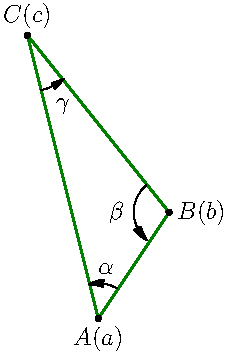
\includegraphics{./C2002_3.pdf}
  \caption{Somme des angles d'un triangle}
  \label{fig:C2002_3}
\end{figure}
Suivant le dictionnaire précédent, on peut interpréter les angles de la figure \ref{fig:C2002_3} comme des arguments de nombres complexes.
\renewcommand{\arraystretch}{1.8}
\begin{tabular}{|l|c|c|c|} \hline
angles            & $\alpha$          & $\beta$           & $\gamma$ \\ \hline
nombres complexes & $\frac{c-a}{b-a}$ & $\frac{a-b}{c-b}$ & $\frac{b-c}{a-c}$ \\ \hline
\end{tabular}

En introduisant les modules $\rho_A$, $\rho_B$, $\rho_C$, on peut écrire
\begin{displaymath}
\left. 
\begin{aligned}
\frac{c-a}{b-a} = \rho_A e^{i\alpha} \\
\frac{a-b}{c-b} = \rho_B e^{i\beta} \\
\frac{b-c}{a-c} = \rho_A e^{i\alpha} \\
\end{aligned}
\right\rbrace 
\Rightarrow
\rho_A \rho_B \rho_C \, e^{i(\alpha + \beta + \gamma)} = \frac{c-a}{b-a}\,\frac{a-b}{c-b}\,\frac{b-c}{a-c} = -1
\Rightarrow \alpha + \beta + \gamma \equiv 0 \mod (2\pi)
\end{displaymath}


\subsection{ Interprétations géométriques de certaines fonctions.}
\begin{itemize}
 \item Soit $u$ un nombre complexe fixé. La transformation du plan qui à tout point $M$ associe le point d'affixe $m+u$ est une translation de vecteur $\overrightarrow u$.
 \item Soit $\theta$ un nombre réel fixé non congru à $0$ modulo $2\pi$ et $a$ un nombre complexe fixé. La transformation du plan qui à tout point $M$ associe le point d'affixe $me^{i\theta}+a$ est une rotation d'angle $\theta$ et de centre le point d'affixe $\frac{a}{1-e^{i\theta}}$.
 \item Soit $u$ unitaire et $\alpha$ un argument de $u$, soit $a$ complexe. L'application 
\begin{displaymath}
 z\rightarrow u(z-a) +a
\end{displaymath}
s'interprète géométriquement comme la rotation d'angle $\alpha$ et de centre $a$.
\item Soit $a$ et $b$ complexes avec $a\neq 0$. La transformation géométrique associée à la transformation complexe
\begin{displaymath}
 z\rightarrow az +b
\end{displaymath}
est une translation lorsque $a=1$, une rotation lorsque $|a|=1$, une homothétie lorsque $a$ est réel et $\neq1$, une similitude dont le rapport est le module de $a$ et l'angle un argument de $a$ lorsque $|a|\neq 1$. Lorsque $a \neq 1$,le centre est le point fixe de la transformation c'est à dire l'unique solution de $z = az +b$.
\end{itemize}

\subsection{ Forme complexe de la formule dite d'Al Kashi.} \index{formule d'Al Kashi}
On considère le triangle formé par les points $O$, $A$, $B$ respectivement d'affixes $0$, $a$, $b$. Notons $\theta$ une mesure de l'angle orienté $(\overrightarrow{OA},\overrightarrow{OB})$ c'est aussi un argument de $\frac{b}{a}$ ou de $b\overline{a}$. L'identité remarquable suivante s'interprète alors comme la forme complexe du théorème d'Al Kashi de terminale:
\begin{displaymath}
 |b-a|^2 = |a|^2 + |b|^2 -2\Re (\overline{a}b) = |a|^2 + |b|^2 -2|a||b|\cos \theta
\end{displaymath}

\begin{figure*}
 \centering
 \input{C2002_1.pdf_t}
 \caption{Forme complexe d'Al Kashi}
 \label{fig:C2002_1}
\end{figure*}

\subsection{Droites}
\subsubsection{\'Equation de droite.}\index{équation de droite}
Si $x$ et $y$ désignent les fonctions coordonnées relatives à un repère orthonormé et $a$, $b$, $c$ sont trois nombres réels tels que $(a,b)\neq(0,0)$. L'équation
\begin{displaymath}
 ax+by+c =0
\end{displaymath}
est l'équation d'une droite. C'est à dire que l'ensemble des points $M$ vérifiant $ax(M)+by(M)+c=0$ est une droite.\newline
Réciproquement, si $\mathcal{D}$ est une droite, il existe $a$, $b$, $c$ réels tels que $(a,b)\neq(0,0)$ et que 
\begin{displaymath}
M\in \mathcal{D} \Leftrightarrow ax(M) + by(M) + c =0
\end{displaymath}
Soit $a$, $b$, $c$, $x$, $y$ des nombres réels quelconques. Alors
\begin{displaymath}
 ax+by+c = \Re(z\overline{u}-c) \text{ avec } z = x+iy \text{ et } u = a+ib 
\end{displaymath}
On en déduit que la forme complexe d'une équation de droite est
\begin{displaymath}
 \Re(z\overline{u}-c) = 0
\end{displaymath}
\subsubsection{Définition paramétrique d'une droite.}
On peut définir une droite $\mathcal{D}$ par un point $A$ affixe $a$ et un vecteur $\overrightarrow{u}$ non nul d'affixe $u$. On peut caractériser l'appartenance à cette droite d'un point quelconque $Z$ d'affixe $z$.
\begin{displaymath}
 Z\in \mathcal{D} \Leftrightarrow \exists t\in \R \text{ tq } z-a = tu
\Leftrightarrow \frac{z-a}{u} \in \R
\Leftrightarrow \text{ les arguments de } \frac{z-a}{u} \equiv 0 \mod \pi
\end{displaymath}
On peut compléter la condition générale d'alignement citée plus haut
\begin{itemize}
 \item $C$ sur la demi droite d'origine $A$ et passant par $b$ si et seulement si $\frac{c-a}{b-a}\in \R_+$.
 \item $C$ sur le segment d'extrémités $A$ et $B$ si et seulement si $\frac{c-a}{b-a}\in [0,1]$.
\end{itemize}
\subsubsection{Alignement de 3 points.}
\begin{prop}\index{alignement de 3 points}
  Trois points distincts $A$, $B$, $C$ d'affixes $a$, $b$, $c$ sont alignés si et seulement si
  \begin{displaymath}
    \frac{b-a}{c-a} \in \R
  \end{displaymath}
\end{prop}
\begin{demo}
  La condition signifie que l'angle entre les vecteurs $\overrightarrow{AC}$ et $\overrightarrow{AB}$ est congru à $0$ modulo $\pi$.
\end{demo}


\subsection{Cercles.}
\subsubsection{\'Equation.}
La forme complexe d'une équation de cercle est complètement naturelle. Un point quelconque $Z$ d'affixe $z$ est sur le cercle de centre $C$ d'affixe $c$ et de rayon $r$ si et seulement si 
\begin{displaymath}
 |z-c| = R
\end{displaymath}
En posant $x=\Re z$ et $y = \Im z$, on obtient une équation du second degré de la forme 
\begin{displaymath}
  x^2 + y ^2 + A x + By + C = 0
\end{displaymath}
où $A$, $B$, $C$ sont des paramètres réels. On remarque qu'il n'y a pas de terme en $xy$ et que les coefficients de $x$ et de $y$ sont égaux.\newline
Réciproquement, lorsqu'une équation de cette forme admet des solutions. Les représentants de ses solutions forment un cercle. Pour l'obtenir, il suffit d'écrire des débuts de carrés:
\begin{displaymath}
x^2 + y^2 + Ax + By + \cdots = (x+\frac{A}{2})^2 + (y+\frac{B}{2})^2 -\frac{A^2}{4} - \frac{B^2}{4} + \cdots  
\end{displaymath}
pour faire intervenir le carré d'un module.

\subsubsection{Inversion et cocyclicité de quatre points.}\index{inversion} \index{cocyclicité de quatre points}
Les résultats présentés dans cette section ne sont pas au programme de MPSI mais constituent de bons exemples de mise en \oe{}uvre des éléments du programme.
\begin{prop}
  Quatre nombres complexes $A$, $B$, $C$, $D$ d'affixes $a$, $b$, $c$, $d$ sont cocycliques (sur un même cercle) si et seulement si :
  \begin{displaymath}
    \frac{(c-b)(d-a)}{(c-a)(d-b)} \in \R
  \end{displaymath}
\end{prop}
\begin{demo}
  La preuve de cette proposition se déduit des résultats suivants.
\end{demo}

On note $\mathcal{I}$ (inversion) l'application du plan privé de l'origine dans le plan privé de l'origine et qui, à tout nombre complexe $z\neq0$ associe $\frac{1}{z}$.\newline
Cette application est clairement une involution c'est à dire qu'elle vérifie $\mathcal{I}\circ \mathcal{I} = Id$.
\begin{prop}
 L'image par $\mathcal{I}$ d'une droite qui ne passe pas par l'origine $O$ est un cercle passant par $O$ mais privé de $O$. L'image par $\mathcal{I}$ d'un cercle passant par $O$ mais privé de $O$ est une droite qui ne passe pas par l'origine $O$.
\end{prop}
\begin{demo}
 Soit $\mathcal{D}$ une droite ne passant pas par $O$. Son équation est de la forme $ax+by+c$ avec $c\neq0$ caractérisant le fait que $O\not\in \mathcal D$.\newline
Soit $Z\neq O$ d'affixe $z$ un point quelconque du plan. Alors 
\begin{displaymath}
 Z\in \mathcal{I}(\mathcal{D})\Leftrightarrow \mathcal{I}(Z)\in \mathcal D
\Leftrightarrow a\frac{\Re(z)}{|z|^2} - b\frac{\Im(z)}{|z|^2} +c =0
\end{displaymath}
car l'affixe de $\mathcal{I}(Z)$ est $\frac{1}{z}=\frac{\overline{z}}{|z|^2}$.
\end{demo}
Notons $u=a+ib$. On a alors
\begin{multline*}
 a\frac{\Re(z)}{|z|^2} - b\frac{\Im(z)}{|z|^2} +c = \frac{\Re(zu)}{|z|^2}+c
= \frac{1}{|z|^2}\left( \Re(zu) + c|z|^2\right)\\
=  \frac{c}{|z|^2}\left( \Re(z\frac{u}{c}) + |z|^2\right)
= \frac{c}{|z|^2}\left(|z+\frac{\overline{u}}{2c}|^2 - \left|\frac{\overline{u}}{2c}\right|^2\right)
\end{multline*}
On en déduit que $\mathcal{I}(\mathcal{D})$ est le cercle de centre le point d'affixe $\frac{\overline{u}}{2c}$ et de rayon |$\left|\frac{\overline{u}}{2c}\right|$. Ce cercle passe par l'origine car le rayon est le module de l'affixe du centre. L'origine n'est pas atteinte par $\mathcal I$.

Application à la cocyclicité de quatre points.\newline
$A$, $B$, $C$, $D$ sont cocycliques si et seulement si les points d'affixes $b-a$, $c-a$, $d-a$ sont sur un cercle qui passe par l'origine si et seulement si les points d'affixes $\frac{1}{b-a}$, $\frac{1}{c-a}$, $\frac{1}{d-a}$sont alignés. \newline
Or
\begin{displaymath}
 \frac{\frac{1}{c-a} - \frac{1}{b-a}}{\frac{1}{d-a}-\frac{1}{b-a}}
=\frac{(b-c)(d-a)}{(c-a)(b-d)}=\frac{(c-b)(d-a)}{(c-a)(d-b)}
=\frac{\frac{c-b}{c-a}}{\frac{d-b}{d-a}}
\end{displaymath}
Finalement: les quatre points $A$, $B$, $C$, $D$ sont cocycliques si et seulement si les arguments de $\frac{c-b}{c-a}$ et de $\frac{d-b}{d-a}$ sont congrus modulo $\pi$.

\begin{figure}[h]
  \centering
  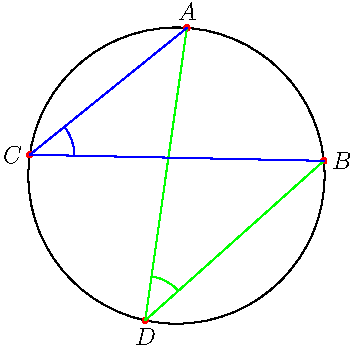
\includegraphics{./C2002_2.pdf}
  % C2002_2.pdf: 170x170 pixel, 72dpi, 6.00x6.00 cm, bb=0 0 170 170
  \caption{points cocycliques}
  \label{fig:C2002_2}
\end{figure}

On en déduit la proposition annoncée au début.

\end{document}
